\documentclass{report}
\usepackage{homework}
\usepackage{url}
\solstrue

\usepackage{graphicx}
\usepackage{pbox}
\graphicspath{{figures/}}

\renewcommand{\hmwkTitle}{Homework 8}

\begin{document}
\mktitle

\begin{problem}
Consider a network of 6 routers shown in the figure below. The network is running OSPF routing protocol and the cost of each link is 10. Each router is announcing a single unique prefix, in total 6 prefixes are announced (prefix A, prefix B, ... prefix F). Propagation delay for each link is 10msec. When a router has to choose between two or more equal cost paths to the same destination, it breaks the tie by picking the path whose next hop has smallest name (A $<$ B $<$ C $<$ D $<$ E $<$ F). The network has been up and running for a long time. However, at time T=100 min, link A-F fails.

\begin{center}
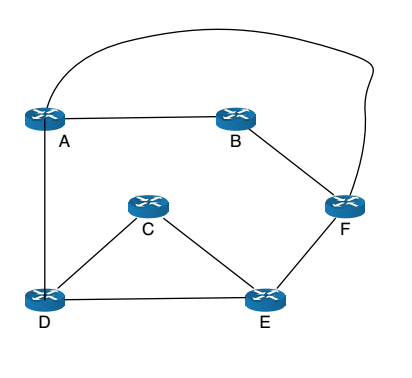
\includegraphics[scale=0.5]{hw8-q1.png}
\end{center}
\begin{enumerate}
\item How do node A and node F discover this link failure? \\ \\

\begin{answer}{5em}
Write your answer here
\end{answer}

\item Will node C learn about this link failure? 
If so, does knowing this failure affect C's forwarding table? \\ \\

\begin{answer}{5em}
Write your answer here
\end{answer}
\end{enumerate}

\end{problem}


\newpage



\begin{problem}
Consider the network shown below. Suppose all ASes (AS 1 -- AS 4) are running OSPF for their intra-AS routing protocol. Suppose BGP is used for the
inter-AS routing protocol (and iBGP is used inside each AS).

\begin{center}
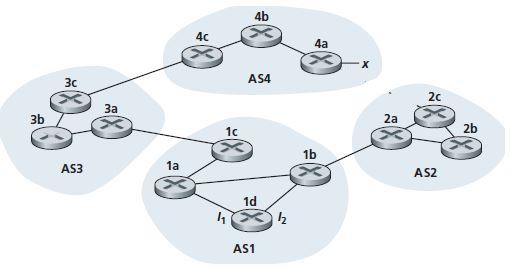
\includegraphics[scale=0.7]{hw8-q2.jpg}
\end{center}

At some time T, the prefix $x$ appears in AS4, adjacent to the router 4a.
From which routing protocol (OSPF, eBGP, or iBGP):

\begin{enumerate}
\item Router 1c learns about prefix $x$? 
\item Router 3b learns about prefix $x$?
\item Router 4a learns about prefix $x$?
\end{enumerate}


\begin{answer}{20em}
Write your answer here
\end{answer}

\end{problem}

\newpage



\begin{problem}
\begin{enumerate}
    \item How does BGP detect loops in paths?
    \item Why does a BGP router not always choose routes with the shortest AS-path length?
\end{enumerate}

\begin{answer}{20em}

    Write your answer here
\end{answer}

\end{problem}

\newpage



\begin{problem}
Suppose four active nodes—nodes A, B, C and D—are competing for access to a channel using slotted ALOHA. Assume each node has an infinite number of packets to send. Each node attempts to transmit in each slot with probability p. The first slot is numbered slot 1, the second slot is numbered slot 2, and so on.

\begin{enumerate}
\item What is the probability that node A succeeds for the first time in slot 5?
\item What is the probability that any node (either A, B,C or D) succeeds in slot 4?
\end{enumerate}

\begin{answer}{45em}
Write your answer here
\end{answer}
\end{problem}


\newpage



\begin{problem}
Consider the following network topology with specified MAC addresses for network interfaces and the configured IP addresses:

\begin{center}
  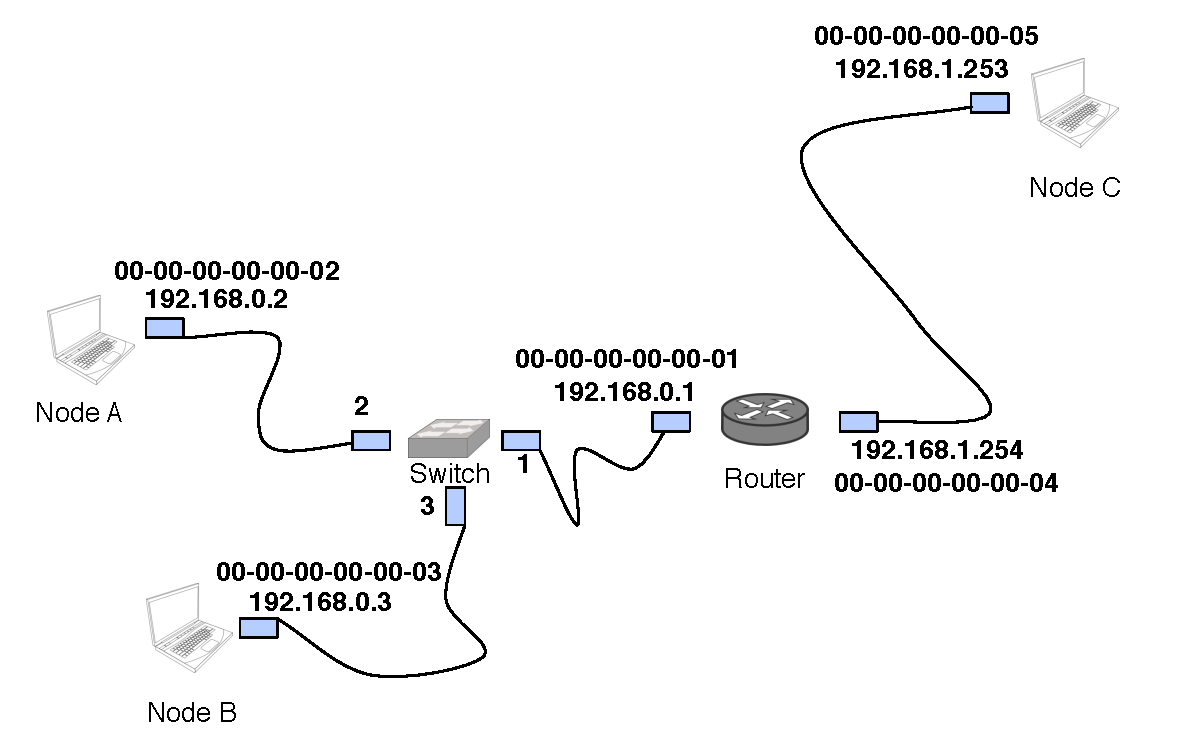
\includegraphics[scale=0.7]{hw8-q5.pdf}
\end{center}

Assume the network mask for both subnetworks is 255.255.255.0.
\begin{enumerate}

  \item Assume that routing tables are properly configured and the network just started (i.e., all caches are empty), fill the following table to enumerate Ethernet frames (in chronological order) needed for node B to send an IP packet to 192.168.0.2 and receive a response back.

  \begin{table}[H]
    \centering
    \begin{tabular*}{1.0\textwidth}{c | c | c | c | c}
      \hline
      frame \# &  dst MAC addr & src MAC addr & \pbox{20cm}{device(s) that can get the frame, \\excluding the sender} & \pbox{20cm}{new entries added into \\the switch's table (if any)} \\ \hline

        &  &  & &\\ 
        &  &  & &\\ 
        &  &  & &\\ 
        &  &  & &\\ 
        &  &  & &\\ 
        &  &  & &\\ 
        &  &  & &\\ 
        &  &  & &\\ 
        &  &  & &\\ 
        &  &  & &\\ 
        &  &  & &\\ 
        &  &  & &\\ 
        &  &  & &\\ 
        &  &  & &\\ 
        &  &  & &\\ 
    \end{tabular*}
  \end{table}

\clearpage
  \item Assume that the previous operation is done,  fill the following table to enumerate Ethernet frames (in chronological order) for node B to send a packet to 192.168.1.253 and receive a reply.
  \begin{table}[H]
    \centering
    \begin{tabular*}{1.0\textwidth}{c | c | c | c | c}
      \hline
      frame \# &  dst MAC addr & src MAC addr & \pbox{20cm}{device(s) that can get the frame, \\excluding the sender} & \pbox{20cm}{new entries added into \\the switch's table (if any)} \\ \hline

        &  &  & &\\ 
        &  &  & &\\ 
        &  &  & &\\ 
        &  &  & &\\ 
        &  &  & &\\ 
        &  &  & &\\ 
        &  &  & &\\ 
        &  &  & &\\ 
        &  &  & &\\ 
        &  &  & &\\ 
        &  &  & &\\ 
        &  &  & &\\ 
        &  &  & &\\ 
        &  &  & &\\ 
    \end{tabular*}
  \end{table}
\end{enumerate}

\end{problem}

\end{document}
